%!TEX root = ../thesis.tex
\chapter{Evaluation}\label{evaluation}


\ifpdf
    \graphicspath{{Chapter3/Figs/Raster/}{Chapter3/Figs/PDF/}{Chapter3/Figs/}}
\else
    \graphicspath{{Chapter3/Figs/Vector/}{Chapter3/Figs/}}
\fi


\NOTE{A}{I am really not sure about the best structure for this chapter.}

\section{General Notes} \label{evaluationnotes}

In this chapter I provide quantitative and qualitative analysis and comparison of the settings presented in previous chapters.


To obtain thorough and statistically significant results\NOTE{D}{You used parallel processing to speed up the executions.}, I utilised parallel processing as much as possible for evaluating Deep Q-Learning policies, which are the bottleneck of the evaluation phase. To exploit the parallelism of the GPU even with the inherently sequential MDP, I ran several (usually $64$) independent samples in parallel. Note that this is much simpler for \TwoThinning and \GraphicalTwoChoice, where the number of steps from start to end\NOTE{D}{remove ``from start to end''?} in the MDP is constant\NOTE{D}{fixed?} ($m$) in any execution.


Even with this evaluation speedup\NOTE{D}{I think here you are interested in two quantities: (i) training time and (ii) time to evaluate the next threshold.}, the usability of Deep Q-Learning for large values of $n$ and $m$ is still limited due to the training time. The largest range for which I successfully trained a RL algorithm in at most a day is $n=1000$, $m=1500$, but I decided to focus on slightly smaller values for the evaluation as that is more illustrative and complementary to the literature available.\NOTE{D}{This sentence should not be needed if there is an appropriate table with timings}


For illustration purposes\NOTE{T}{Isn't it more for space reasons?} I will usually pick out a specific value\NOTE{D}{I will choose some representative values} of $n$ and $m$\NOTE{D}{to illustrate the general trends (and remove ``but..''}, but my conclusions hold in general, unless I state otherwise.

\NOTE{A}{TODO: Note that in this project there is no train or test set, there isn’t any data at all. Nevertheless, it is still important to do evaluation independently of early stopping, due to the Expectation-Maximum Jensen inequality.}


\NOTE{D}{You need a bullet point overview of the evaluations here.}

\section{Two-Thinning}


\subsection{Comparison of Strategies}

Now I present a comparison of seven \TwoThinning strategies. I have chosen nine combinations of $n$ (number of bins) and $m$ (number of balls) so that they cover different ranges, and also different balls-bins ratios \NOTE{T}{maybe ``average loads''(?)}\NOTE{D}{Repetition. Mention it either here or in the previous section.}.


To have acceptable statistical significance but also reasonable runtime, I compared the strategies across $100$ runs. I show the average of scores (maximum load) of the runs and also the $95\%$ confidence interval for the estimated mean score, based on the Central Limit Theorem (CLT). \NOTE{A}{Should I explain more? Any formal statistical reason for choosing the number of runs?}


Note that the Dynamic Programming (DP) Strategy is optimal by definition, but it is too slow for larger values of $n$ and $m$ which I denote by TLE (Time Limit Exceeded)\NOTE{D}{Time Limit Exceeded (TLE)}. I decided to limit all the algorithms to $12$ hours of training/preparation, declaring anything above that as TLE.\NOTE{D}{The limit was set to $12$ hours of training/precomputation.} Also, even though we have the exact expected maximum load of the DP Strategy, I decided to run it just like the other strategies for fair comparison (e.g.\ large outliers that the DP Strategy takes into account occur very rarely during execution).


For the Threshold Strategy, I calculated the optimal values by modelling it as a Multi-Armed Bandit problem (covered in II Randomised Algorithms) \cite{katehakis1987multiarmedbandit}, and using an $\epsilon$-greedy strategy with $\epsilon=0.1$ (details omitted).


I note that there is merit in not just doing several runs with the trained trained Deep Q-Learning model, but also retraining it several times (e.g.\ $20$ runs with each of $5$ independently trained model), because the rewards received during training are also probabilistic\NOTE{D}{This should not matter if the algorithm is trained for long enough, right? Also, it is more standard that you train multiple models and you keep one (by seeing its performance on evaluation data. And this one you thoroughly test.}. This idea would rather evaluate the robustness of the Deep Q-Learning framework for balls-into-bins settings, but I decided to stick to a single trained model and essentially evaluate the peak performance. \NOTE{A}{Does it make any sense? This idea came to my mind and I am a bit unsure about it and couldn't find any reference.} \NOTE{T}{It makes some sense... But again I would then make the random bin choices identical for all these runs.}. Relatedly, one could consider finding the optimal hyperparameters as a special part of training, but I decided treat it separately, and in particular, not take it into account for the $12$ hour TLE limit.\NOTE{D}{I don't understand this sentence.}


\begin{table}[h!]
\label{tab:two-thinning-comparison}
\centering
\resizebox{\textwidth}{!}{%
\begin{tabular}{|l|c|c|c|c|c|c|c|c|c|}
\hline
                                & \multicolumn{3}{c|}{$n=5$} & \multicolumn{3}{c|}{$n=20$} & \multicolumn{3}{c|}{$n=50$} \\ \hline
Strategy                                & $m=5$ & $m=10$ & $m=25$ & $m=20$ & $m=60$ & $m=400$ & $m=50$ & $m=200$ & $m=2500$ \\ \hline
Always Accept & 2.26 $\pm$ 0.06 & 3.84 $\pm$ 0.10 & 7.88 $\pm$ 0.14 & 3.26 $\pm$ 0.10 & 6.68 $\pm$ 0.15 & 28.84 $\pm$ 0.32 & 3.87 $\pm$ 0.10 & 9.12 $\pm$ 0.16 & 66.66 $\pm$ 0.50 \\ \hline
Random & 2.35 $\pm$ 0.07 & 3.72 $\pm$ 0.09 & 7.66 $\pm$ 0.14 & 3.21 $\pm$ 0.10 & 6.67 $\pm$ 0.15 & 28.55 $\pm$ 0.32 & 3.80 $\pm$ 0.10 & 9.02 $\pm$ 0.18 & 66.83 $\pm$ 0.48 \\ \hline
Local Reward Optimiser & 1.82 $\pm$ 0.05 & 2.97 $\pm$ 0.05 & 6.08 $\pm$ 0.06 & 2.25 $\pm$ 0.06 & 4.75 $\pm$ 0.08 & 22.46 $\pm$ 0.09 & 2.54 $\pm$ 0.07 & 6.37 $\pm$ 0.07 & 53.98 $\pm$ 0.11 \\ \hline
Mean Thinning & 1.87 $\pm$ 0.07 & 3.10 $\pm$ 0.07 & 6.17 $\pm$ 0.09 & 2.56 $\pm$ 0.08 & 5.12 $\pm$ 0.10 & 22.52 $\pm$ 0.12 & 3.06 $\pm$ 0.08 & 6.79 $\pm$ 0.11 & 53.53 $\pm$ 0.15 \\ \hline
DP & 1.85 $\pm$ 0.06 & 2.98 $\pm$ 0.07 & 6.06 $\pm$ 0.10 & 2.33 $\pm$ 0.10 & 4.69 $\pm$ 0.11 & TLE & 2.52 $\pm$ 0.10 & TLE & TLE \\ \hline
Deep Q-Learning & 1.92 $\pm$ 0.09 & 2.93 $\pm$ 0.09 & 6.20 $\pm$ 0.11 & 2.42 $\pm$ 0.10 & 4.88 $\pm$ 0.12 & 22.20 $\pm$ 0.14 & 2.50 $\pm$ 0.11 & 6.43 $\pm$ 0.11 & 53.49 $\pm$ 0.25 \\ \hline
Threshold & 2.18 $\pm$ 0.13 & 3.32 $\pm$ 0.13 & 6.44 $\pm$ 0.13 & 2.58 $\pm$ 0.12 & 5.58 $\pm$ 0.17 & 24.12 $\pm$ 0.19 & 2.99 $\pm$ 0.12 & 7.02 $\pm$ 0.13 & 56.73 $\pm$ 0.29 \\ \hline 

\end{tabular}}
\caption{Average maximum load of \TwoThinning strategies with $95\%$ confidence intervals}
\end{table}
\NOTE{D}{Which method did you use to generate the confidence intervals?}
\NOTE{D}{Maybe highlight the top three results from each column?}

\NOTE{D}{Maybe it is best to summarise the key observations from each table/figure in a bullet point list.}
We can see that the Always Accept\NOTE{D}{Define commands for these, e.g.\ \textsc{Always-Accept}} and Random Strategies are consistently poorly performing. The DP Strategy is not shown\NOTE{T}{Do you want to drop the word ``shown''?} to be exactly the best for reasons outlined above. The Threshold Strategy, even though asymptotically shown to be optimal is outperformed by several other strategies. The difference is even more significant for larger $m$, when the constant threshold (on the primary allocations) is too much of a restriction. The Mean Thinning, Local Reward Optimiser and Deep Q-Learning Strategies seem to be comparable to each other. I have calculated the one-sided p-values of a two sample t-test to see if the Deep Q-Learning Strategy is significantly better than the Mean Thinning Strategy for larger values of $n$ and $m$. The difference is significant for most of the cases (the p-values are $\sim 10^{-3}$ for $n=20$,\NOTE{T}{maybe replace these commas by and, otherwise it is very hard to parse.} $m=400$, $\sim 10^{-17}$ for $n=50$, $m=50$, $\sim 10^{-5}$ for $n=50$, $m=200$) but more data would be required for $n=50$, $m=2500$. \NOTE{A}{Double check that I am not writing something stupid. In particular, the test I applied assumes that the maximum loads are from a normal distribution and the two distributions have the same variance and none of them are actually true, at least not exactly... How to remedy this?} \NOTE{A}{Should I do some more p-values or this is enough to convince them about the professionalism of this dissertation?}

\NOTE{A}{Should I say some more, clever bullshit about the table, some general patterns, etc.? Maybe a bit more about the difference between the columns, not between the rows.}
\NOTE{D}{Maybe mention all analysis techniques and why they are suitable for these settings in the introduction. So, here you would only mention the p values }


One of the main surprises of the comparison is that the Local Reward Optimiser Strategy (which rejects only the maximum loads) has similar performance as the Deep Q-Learning Strategy, which was trained to optimise cumulative rewards. This suggests that the RL problem underlying \TwoThinning is a challenging one, in particular, learning long-term consequences of decisions is difficult, because the impact of a single ball is very subtle. In general, making a small number of bad decisions might not even impact the final maximum load. \NOTE{A}{TODO: elaborate some more? This is a crucial point to make.}\NOTE{T}{Isn't one of the reasons of why the local reward optimiser is so good that you cannot scale up $n$ and $m$ too much?}


\NOTE{A}{Write a bit about the running time of both training and evaluation. DQN would be a bit slower latency-wise but it is bearable. Note that other strategies require no training.}



\NOTE{A}{Add plot showing that it doesn't work very well for larger $n$ and $m$. Add general plots for huge $n$ and $m$. Also I can include here the tendencies for the theoretical results, e.g.\ plotting a logarithmic curve. Mention the difficulty in finding the constant factor of those theoretical algorithms.}

\subsection{Optimal Strategy Analysis}

\NOTE{D}{Maybe you could call this ``Theoretical analysis''}
Analysing the optimal strategies for \TwoThinning, I formulated the following lemma.

\begin{lemma}\label{lemma: two-thinning-increasing-threshold}
The chosen thresholds of an optimal protocol are non-decreasing during an execution. That is, if for $i$th\NOTE{T}{for the $i$-th} ball the protocol chooses a threshold $x$, then for every $j$th ball of the same game\NOTE{T}{replace game by process or execution} such that $j>i$, a threshold $y\geq x$ is chosen.
\end{lemma}


\begin{figure}[hbt!] \label{dp-increasing-threshold}
    \centering
    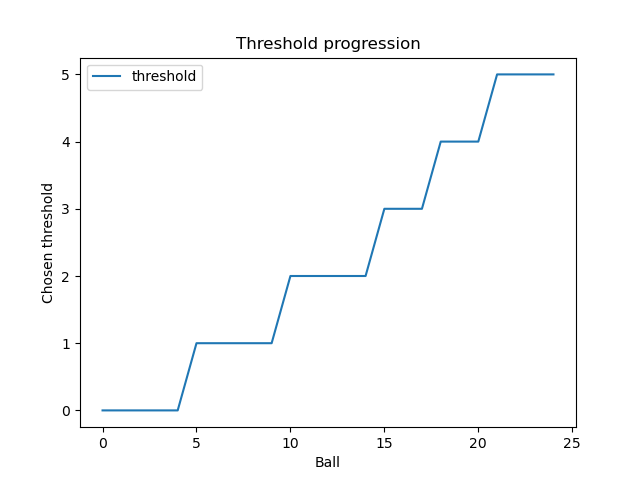
\includegraphics[scale=1.0]{Chapter4/Figs/dp_increasing_threshold.png}
    \caption{A run of the DP Strategy showing the increasing threshold property}
\end{figure}
\NOTE{D}{!!I think this figure on its own does not show much. Maybe you could add several executions with different colours, so that the reader sees the trend. Also it would be nice if you had runs for different initial configurations (e.g.\ starting with one bin and a maximum load of $5$ or half the bins having a maximum load of $5$. This would be part of a ``thorough'' qualitative evaluation. If would spot a trend it would also be nice to support it with some quantitative data.}
This is a very surprising lemma, because the theoretically asymptotically optimal protocols\NOTE{T}{Why protocols? I guess here you can refer to the one protocol used in one of the Feldheim papers?} in the literature do not have this property. We think that this is because they are optimal only up to a constant (or logarithmic) factor, and they are easier to reason about analytically and prove bounds on them (usually these protocols consist of independent phases with different behaviour).


\begin{proof}

\NOTE{A}{Do proper proof.}
\NOTE{T}{Do we really think we have a proof of that?}

The lemma has been verified by the optimal strategy(s) generated by dynamic programming, for several combinations of $n$ and $m$. 
\end{proof}

To get a deeper understanding of the optimal (DP) strategy, I analysed the probability of it reaching different states (sorted load vectors)\NOTE{D}{!!Always reference the figure!!} during an execution of the game (I used another DP algorithm for this). I present the following analysis for the $n=20$, $m=20$ case, but the same observations hold for other cases as well.

\NOTE{D}{Again, maybe a bullet list would help}The main observation is that there is a big gap between the probabilities of reaching different states by the optimal strategy. For example, the most likely final state $(0, 0, 0, 0, 0, 0, 1, 1, 1, 1, 1, 1, 1, 1, 2, 2, 2, 2, 2, 2)$ has a probability of almost a quarter, which is very large among $627$ possible final states. The entropy of the probabilities of the final states is $\sim 3.36$, which is nearly a third of the entropy of a uniform distribution with a same number of states\NOTE{D}{Maybe you could give an explicit calculation and perhaps mention that it is smaller than simulation entropy?}. Extending these probabilities to intermediate states as well, we get the following distribution of the probabilities \NOTE{A}{Try to fit a well-known distribution to it!}:
\NOTE{T}{I think you may get a similar distribution if you do the following experiment. You sample $n$ times, independently from a normal distribution $N(0,\sigma)$. A few combinations, e.g., $(0,\ldots,0)$ have the highest probability, but most combinations are like $(\pm \sigma,\pm \sigma)$ etc, which may correspond to your peak around $-50$.}

\NOTE{T}{I'm not sure the figure is really well explained? One interesting phenomena in the chart is that the threshold is increased more often towards the end than towards the beginning.}

\NOTE{T}{I think it is a general rule that every Figure and Table should be refered to as in the main text.}

\begin{figure}[hbt!] \label{two-thinning-state-distribution}
    \centering
    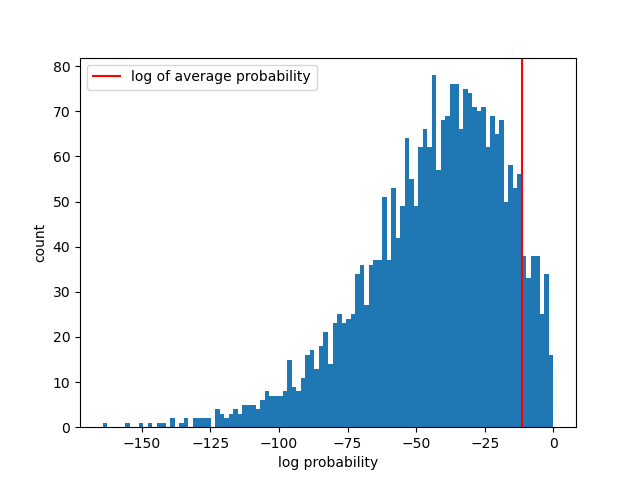
\includegraphics[scale=1.0]{Chapter4/Figs/state_distribution_20_20_all_log_count.png}
    \caption{The distribution of the probabilities of the states for $n=m=20$, using the DP strategy. Due to the skewness of the distribution, the values are shown on a log-scale.}
\end{figure}


In future work, the presence of many small probability states could be exploited to optimise the training of RL algorithms, e.g.\ to find the most relevant curriculum for curriculum learning. 


In many real-world applications it does not suffice if the maximum load is low in expectation, the variance of the maximum load should also be small\NOTE{D}{Maybe ``it should also be small with high probability'' or ``concentrated around the mean''}. Agreeing with theoretical results for other strategies (e.g.\ Threshold Strategy), the DP strategy also has a centralised distribution of the final maximum load:\NOTE{D}{Maybe replace this sentence with ``(in accordance to Section ??)''}


\begin{figure}[hbt!] \label{two-thinning-maxload-distribution}
    \centering
    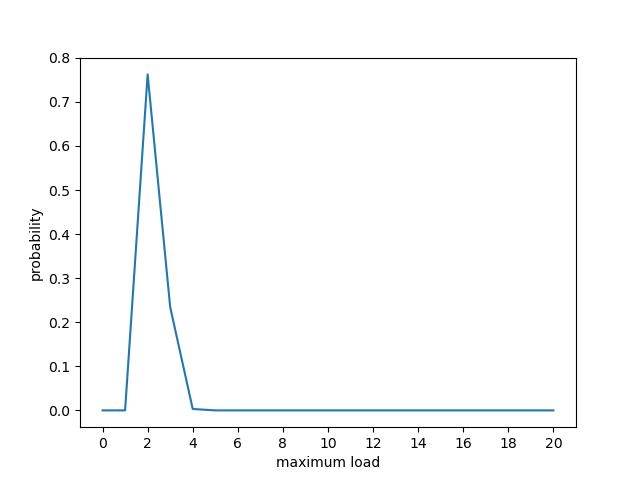
\includegraphics[scale=1.0]{Chapter4/Figs/max_load_distribution_20_20.png}
    \caption{The distribution of the maximum loads for $n=m=20$, using the DP strategy.}
\end{figure}
\NOTE{D}{Maybe use log probability plot as above?}
\NOTE{D}{You could also add plots for several values of $m$ or of $n$.}

% Say something about optimising other objective functions, not the maximum load? Say that it is very hard for RL to learn at such a granular level.



\subsection{Deep Q-Learning analysis}



\NOTE{A}{Maybe add an analysis of Threshold ``Spikes'' During Training and During Execution}



\subsubsection{Hyperparameter Analysis}

\NOTE{A}{Compare zero potential with max load potential, showing P value that we do need reward shaping.}


The Weights and Biases tool provides an analysis of the importance of hyperparameters. It calculates the correlation coefficient between the hyperparameters and the score for each hyperparameter (green is positive, red is negative). To capture interactions between hyperparameters and also non-linear relationships, it also provides an importance score which is calculated based on Random Forests \cite{biewald2020wandb}.


I present the hyperparameter importance analysis\NOTE{D}{Mention which figure} of $200$ runs for the $n=20$ and $m=40$ case, \NOTE{D}{which is indicative of the other cases too}but the pattern is similar for other cases too.


\begin{figure}[hbt!] \label{two-thinning-hyperparameter-importance}
    \centering
    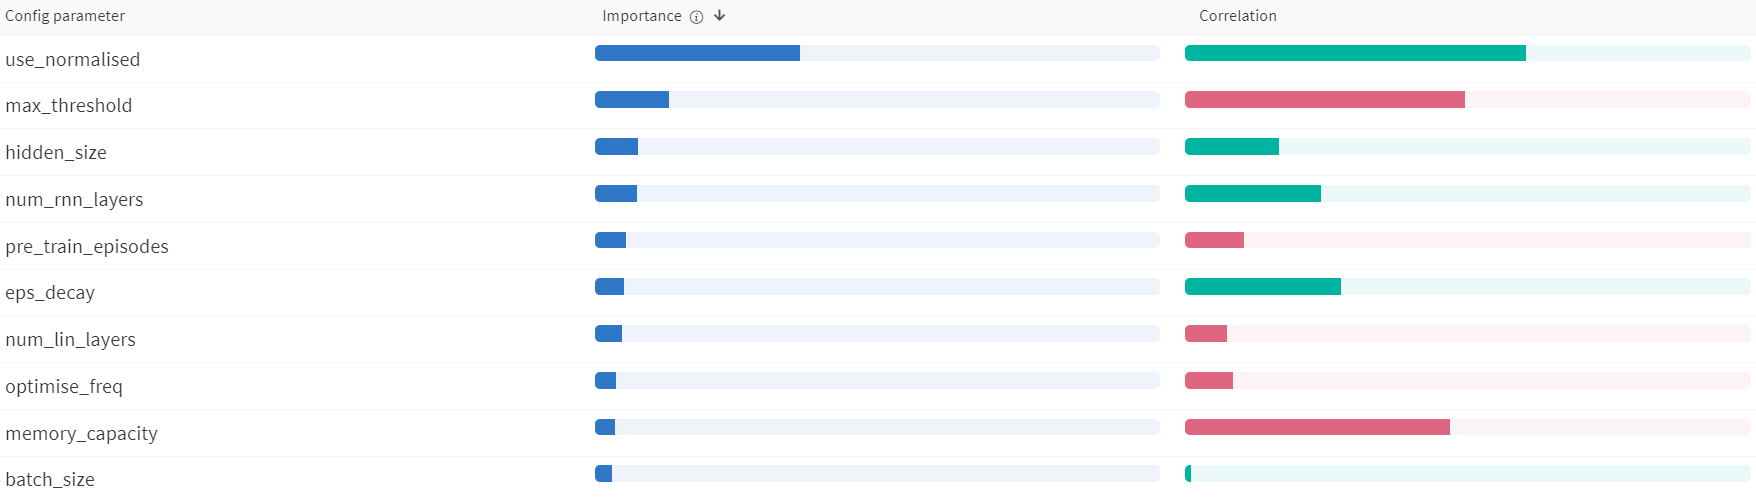
\includegraphics[scale=0.4]{Chapter4/Figs/Hyperparameter_importance_20_400.png}
    \caption{\TwoThinning Hyperparameter Importance}
\end{figure}
\NOTE{T}{very hard to read...}
\NOTE{D}{Again, summarise in bullet points}
We can see that the most important hyperparameter is to use the normalised domain. As discussed earlier, this helps because in the normalised domain, a constant threshold is already a reasonable strategy (see e.g.\ Mean Thinning). Also, limiting the maximum threshold that the agent can use restricts the search space, and fosters learning. As can be seen in Appendix \ref{hyperparameters}, the ideal maximum threshold is around the target expected maximum load we want to achieve (which can be estimated based on theoretical results).



\subsubsection{Training}


\begin{figure}[hbt!] \label{two-thinning-training-curve}
    \centering
    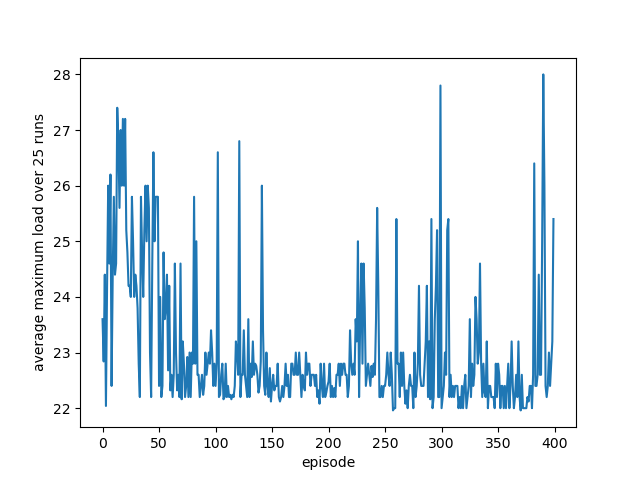
\includegraphics[scale=1.0]{Chapter4/Figs/training_progression_20_400.png}
    \caption{\TwoThinning Training Curve $n=20$, $m=400$}
\end{figure}
\NOTE{T}{Maybe if you do some averaging to the plot, one could see a bit more the learning progress. For example, you could take the average maximum load over the first $x$ episodes.}

We can see that the improvement during training decays very quickly, and the agent is close to its best already at the start. This is again due to the normalised load domain outlined above - I plotted the training curve without the normalised load domain trick, and that shows a much more usual training progression, though leading to a worse optimum. The oscillations are due to both the inherent randomness in evaluation and the agent trying to change its policy in a wrong way.


Motivated by the fact that in the normalised domain, a constant $0$ threshold is the Mean Thinning Strategy, I tried to see if this simple strategy can be improved by choosing another constant ``offset'', not $0$.:\NOTE{D}{Refer to the figure rather than using ``:''}

\begin{figure}[hbt!] \label{two-thinning-constant-offset}
    \centering
    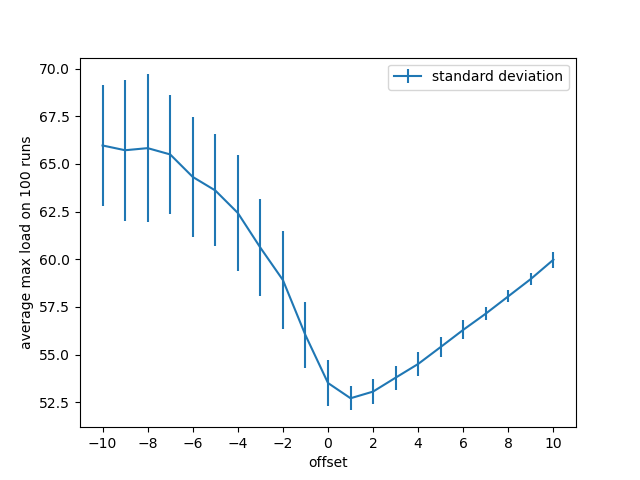
\includegraphics[scale=1.0]{Chapter4/Figs/offset_analysis_50_2500.png}
    \caption{Comparing constant offset strategies for $n=50$, $m=2500$.}
\end{figure}

\NOTE{T}{Very nice! So just to be clear, here are you are comparing different constant offset strategies, and there is no reinforcement learning? I think in one paper, they call this relative threshold strategies. I am wondering a bit what happens if the offset is even smaller. At some point we would reach OneChoice, and perhaps we are already quite close to it. Maybe worth to show that average maxload for OneChoice?}

\NOTE{T}{Another interesting ``philosophical'' insight from the figure seems to be that having a too small offset is more detrimental than having a too large offset.}

\NOTE{D}{!!Can you also try $n = 10^4$ and $m = 10^6$ (or larger)?}

On the figure we can see that for $n=50$, $m=2500$, the best offset is $1$. It holds for general $n$ and $m$ that the best offset is usually slightly above $0$.

The Deep-Q Learning algorithm, which is as shown above, statistically significantly better than Mean-Thinning, actually often learns a strategy close to a constant offset strategy.


\begin{figure}[hbt!] \label{two-thinning-dqn-thresholds}
    \centering
    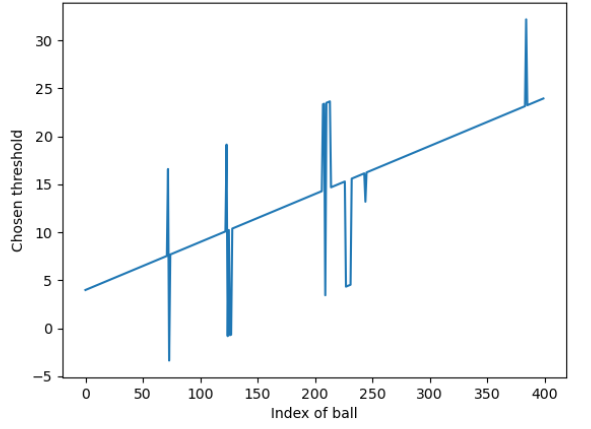
\includegraphics[scale=1.0]{Chapter4/Figs/dqn_learnt_thresholds.png}
    \caption{Analysis of the chosen thresholds of the Deep Q-Learning Strategy for $n=20$, $m=400$. Note that this plot shows only a single run, and the actual load vectors are not displayed.}
\end{figure}

\NOTE{T}{Why do you have this figure here? I don't understand why there is no second threshold in the figure.}


The sporadic ``jumps''\NOTE{T}{So by jumps you refer to the standard deviations bar in Figure 4.6?} are very challenging for the agent to get rid of, because as discussed above\NOTE{D}{where?}, \NOTE{D}{since}a few bad decisions don't have strong impact on the result. To avoid this, as future work the agent could be constrained to change the threshold at most by $1$ after each ball (we have empirical evidence for this to hold for any optimal strategy\NOTE{D}{where?}).



\section{K-Thinning}



\subsection{Comparison of Strategies}


Since the drawback (TLE) of the DP Strategy has already been highlighted for \TwoThinning, I decided to focus on smaller cases here where a full comparison is feasible and highlight other patterns related to the value of $K$.


\NOTE{T}{make $k$ and $K$ more consistent}
\begin{table}[h!]
\label{tab:k-thinning-comparison}
\centering
\resizebox{\textwidth}{!}{%
\begin{tabular}{|l|c|c|c|c|c|c|c|c|}
\hline
                                & \multicolumn{4}{c|}{$n=5$} & \multicolumn{4}{c|}{$n=25$}\\ \hline
                                & \multicolumn{4}{c|}{$m=20$} & \multicolumn{4}{c|}{$m=50$}\\ \hline
Strategy                                & $k=2$ & $k=3$ & $k=5$ & $k=10$ & $k=2$ & $k=3$ & $k=5$ & $k=10$ \\ \hline
Always Accept & 7.82 $\pm$ 0.25 & 7.70 $\pm$ 0.25 & 7.70 $\pm$ 0.24 & 7.73 $\pm$ 0.24 & 5.81 $\pm$ 0.18 & 5.94 $\pm$ 0.19 & 5.85 $\pm$ 0.21 & 6.05 $\pm$ 0.23 \\ \hline
Random & 7.69 $\pm$ 0.26 & 7.62 $\pm$ 0.23 & 7.69 $\pm$ 0.23 & 7.70 $\pm$ 0.23 & 6.02 $\pm$ 0.24 & 5.86 $\pm$ 0.22 & 5.83 $\pm$ 0.20 & 5.70 $\pm$ 0.18 \\ \hline Local Reward Optimiser & 6.12 $\pm$ 0.10 & 5.73 $\pm$ 0.09 & 5.42 $\pm$ 0.10 & 5.13 $\pm$ 0.07 & 4.11 $\pm$ 0.09 & 3.73 $\pm$ 0.09 & 3.21 $\pm$ 0.08 & 3.00 $\pm$ 0.00 \\ \hline
Quantile & 6.24 $\pm$ 0.12 & 6.01 $\pm$ 0.05 & 5.60 $\pm$ 0.10 & 5.16 $\pm$ 0.07 & 4.39 $\pm$ 0.14 & 3.76 $\pm$ 0.11 & 3.15 $\pm$ 0.08 & 3.00 $\pm$ 0.00 \\ \hline
DP & 6.09 $\pm$ 0.09 & 5.69 $\pm$ 0.09 & 5.41 $\pm$ 0.10 & 5.12 $\pm$ 0.06 & 4.15 $\pm$ 0.08 & 3.50 $\pm$ 0.10 & 3.16 $\pm$ 0.07 & 3.00 $\pm$ 0.00 \\ \hline
Deep Q-Learning  & 6.34 $\pm$ 0.15 & 6.08 $\pm$ 0.12 & 5.83 $\pm$ 0.15 & 5.20 $\pm$ 0.08 & 4.44 $\pm$ 0.12 & 4.02 $\pm$ 0.10 & 3.46 $\pm$ 0.10 & 3.01 $\pm$ 0.02 \\ \hline 
Threshold & 6.67 $\pm$ 0.15 & 6.31 $\pm$ 0.11 & 6.08 $\pm$ 0.07 & 5.95 $\pm$ 0.09 & 4.45 $\pm$ 0.12 & 4.18 $\pm$ 0.08 & 4.01 $\pm$ 0.07 & 3.94 $\pm$ 0.08 \\ \hline
\end{tabular}}

\caption{Average maximum load of \KThinning strategies with $95\%$ confidence intervals}
\end{table}

\NOTE{D}{It would also be nice to plot the maximum load for optimal $k$-Thinning or show how the probability distribution changes for different values of $k$.}
Intuitively, the larger $k$ is, the better a strategy can do, and the table confirms it for most of the strategies. We can see from the table that the Quantile and Local Reward Optimiser strategies are almost as good as the DP Strategy for most values of $n$, $m$ and $k$, even though neither of those strategies consider future rewards. For large $k$ ($5$ or $10$) and not too large $n$, strategies can control with high probability where to place the ball. Nevertheless, this kind of advantage is much easier to exploit by a manual algorithm, than to learn by Deep Q-Learning.



Now I present an intuitive lemma about any optimal strategy.


\begin{lemma} \label{lemma: k-thinning-increasing-threshold}
In an optimal strategy, it is not possible that it would accept a bin with $x$ choices left, but reject the same bin (with the same loads) with $y<x$ choices left. In other words, an optimal strategy should never become more selective after rejecting some options.
\end{lemma}


\begin{proof}
Note that Lemma \ref{lemma: thresholdproperty} generalises to \KThinning as well - an optimal strategy must base its decisions on a threshold.


\NOTE{A}{TODO: add real proof}.


Using the dynamic programming algorithm, that creates the optimal strategy(s), I verified the lemma, that is that the threshold is indeed non-decreasing within the same load configuration.
\end{proof}


\subsection{Deep Q-Learning analysis}



\subsubsection{Hyperparameter Analysis}


\begin{figure}[hbt!] \label{k-thinning-hyperparameter-analysis}
    \centering
    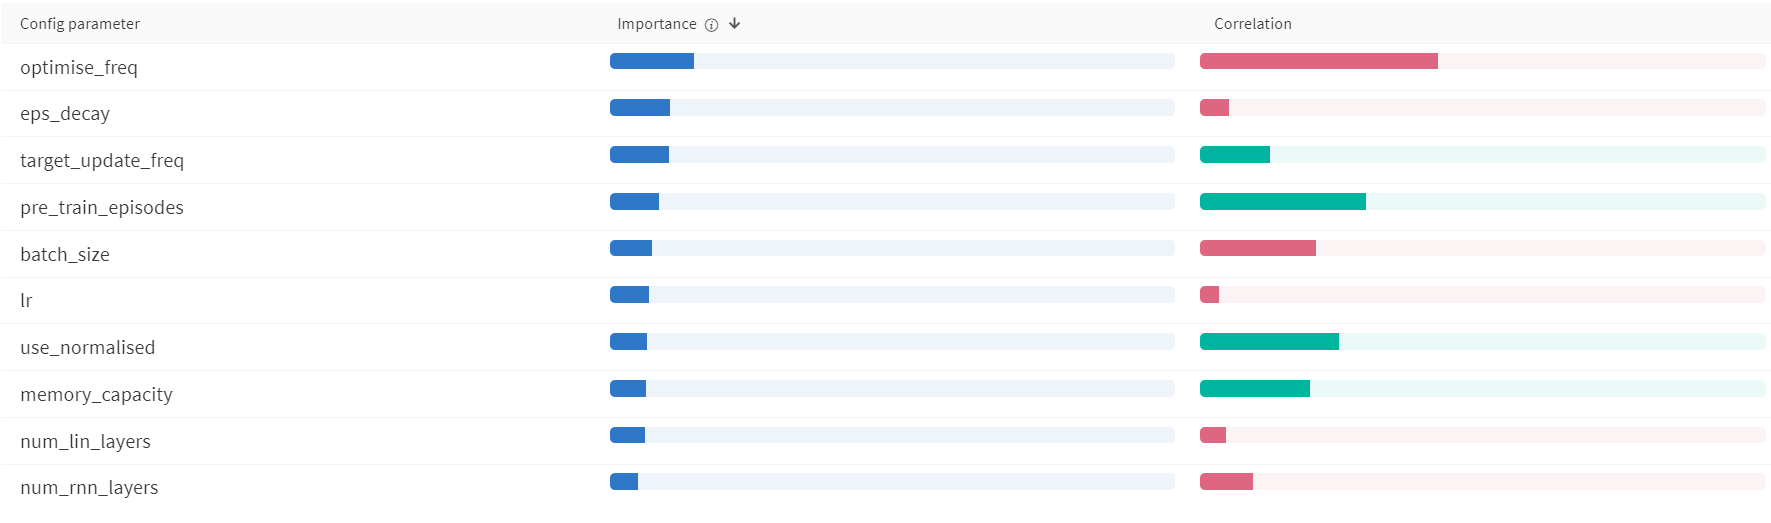
\includegraphics[scale=0.4]{Chapter4/Figs/Hyperparameter_analysis_5_25_3.png}
    \caption{Hyperparamter Importance Analysis for \KThinning with $n=5$, $m=25$, $k=3$.}
\end{figure}

We can observe that Deep Q-Learning cannot exploit the normalised load domain trick for \KThinning as much as for \TwoThinning.\NOTE{A}{Mention some bullshit possible reason?}  On the other hand, the analysis suggests more frequent optimisation update steps and more curriculum learning (pretraining) episodes. 


\subsubsection{Training}


\begin{figure}[hbt!] \label{k-thinning-training-curve}
    \centering
    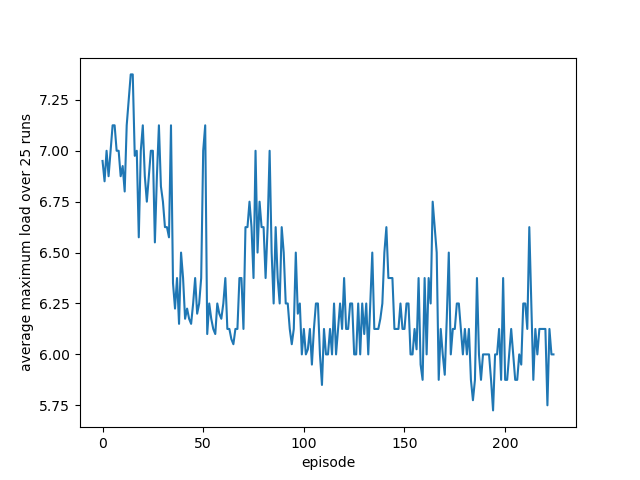
\includegraphics[scale=1.0]{Chapter4/Figs/training_progression_5_25_3.png}
    \caption{\KThinning Training Curve $n=5$, $m=25$, $k=3$. \protect \footnotemark }
\end{figure}


\footnotetext{The last 800 episodes are not shown, as no more significant improvement has happened.}

The training progression for \KThinning is very similar to \TwoThinning, so I don't discuss it any further.


\section{Graphical Two-Choice}


\subsection{Comparison of Strategies}
\begin{table}[h!]
\label{tab:graphical-two-choice-comparison}
\centering
\resizebox{\textwidth}{!}{%
\begin{tabular}{|l|c|c|c|c|c|c|c|c|c|}
\hline
                                & \multicolumn{3}{c|}{$n=4$} & \multicolumn{3}{c|}{$n=16$} & \multicolumn{3}{c|}{$n=32$}\\ \hline
                                & \multicolumn{3}{c|}{$m=25$} & \multicolumn{3}{c|}{$m=50$} & \multicolumn{3}{c|}{$m=32$}\\ \hline
Strategy                                & Cycle & Hypercube & Complete & Cycle & Hypercube & Complete & Cycle & Hypercube & Complete \\ \hline
Greedy & 7.04 $\pm$ 0.03 & 7.04 $\pm$ 0.03 & 7.17 $\pm$ 0.06 & 4.74 $\pm$ 0.08 & 4.47 $\pm$ 0.11 & 4.39 $\pm$ 0.07 & 2.46 $\pm$ 0.10 & 2.34 $\pm$ 0.09 & 2.26 $\pm$ 0.06 \\ \hline
Random & 8.92 $\pm$ 0.17 & 8.81 $\pm$ 0.18 & 8.98 $\pm$ 0.17 & 6.75 $\pm$ 0.17 & 6.64 $\pm$ 0.23 & 6.56 $\pm$ 0.15 & 3.45 $\pm$ 0.13 & 3.64 $\pm$ 0.16 & 3.54 $\pm$ 0.10 \\ \hline
Local Reward Optimiser & 7.10 $\pm$ 0.04 & 7.12 $\pm$ 0.05 & 7.29 $\pm$ 0.07 & 4.97 $\pm$ 0.10 & 4.74 $\pm$ 0.12 & 4.75 $\pm$ 0.07 & 2.53 $\pm$ 0.11 & 2.42 $\pm$ 0.10 & 2.46 $\pm$ 0.07 \\ \hline
DP & 7.01 $\pm$ 0.02 & 7.01 $\pm$ 0.02 & 7.27 $\pm$ 0.10 & TLE & TLE & TLE & TLE & TLE & TLE \\ \hline
Deep Q-Learning & 7.17 $\pm$ 0.07 & 7.17 $\pm$ 0.06 & 7.38 $\pm$ 0.09 & 4.92 $\pm$ 0.15 & 5.71 $\pm$ 0.17 & 6.57 $\pm$ 0.15 & 3.81 $\pm$ 0.18 & 3.59 $\pm$ 0.18 & 4.17 $\pm$ 0.14 \\ \hline  \hline 

\end{tabular}}

\caption{Average maximum load of \GraphicalTwoChoice strategies with $95\%$ confidence intervals\protect\footnotemark}
\end{table}

\footnotetext{Note that for $n=4$, Cycle and Hypercube are the same graphs.}

First I prove the most surprising result of this section.

\begin{lemma} \label{lemma: greedy-suboptimal}
There exist a graph, such that the Greedy strategy is suboptimal with respect to the expected final maximum load of \GraphicalTwoChoice.
\end{lemma}

\NOTE{T}{Make the proof more formal and concise. Information on how you found this using DP is distracting, and I would move it outside the proof. Also maybe the proof is easier to verify if you have a more structured description (figure?) of the load vector and the possible choices/future states.}
\begin{proof}
It is enough to show that there is a state $s$ (i.e.\ a load vector $v$, edge $e$) where is is better to choose the bin with the larger load. This suffices because there is a non-zero probability of reaching $s$, and hence a strategy which agree with Greedy everywhere else except for this state has a strictly better expected score.


I used the dynamic programming algorithm to find the optimal strategy for \GraphicalTwoChoice, and then I searched the strategy for a state where it disagrees with Greedy. I found a very small counterexample for the Cycle graph with $n=4$ bins $m=6$ balls. Denoting the nodes as ($1$-based) indices in the load vector, the counterexample state is $l=(2,0,1,0)$, \NOTE{A}{Change order into 0,a,0,b to make it consistent with the extension later.} $e=(2,3)$,\NOTE{D}{Would it make sense to add a figure here?} i.e.\ there is an edge between the second and third bin. The reason why it is better to choose bin $3$ even though it has larger load than bin $2$ is that after that, from load vector $(2,0,2,0)$ with $2$ balls remaining we can definitely avoid having a maximum load $3$ by always placing the ball in an even-indexed bin. On the other hand, from load vector $(2,1,1,0)$, if both of the remaining edges are $(1,2)$, then there will be a maximum load of at least $3$ using whatever strategy. Therefore, the expected final maximum load of choosing bin $3$ is $2.0$, while that of bin $2$ is between $2.0$ and $3.0$.
\end{proof}\NOTE{D}{Any ideas if this can be generalised for any cycle of length $n$?}



We can see from the table\NOTE{D}{Table ?? shows that}, that for $n=4$ and $m=25$, even though Greedy is not optimal for the Cycle graph but\NOTE{D}{remove but} it is for the Clique\NOTE{D}{Do you need clique and cycle with capital?} graph, the optimal strategy for the Cycle graph (provided by the DP Strategy) still has a lower expected maximum load than Greedy has for the Clique graph. This is an important observation, because it indicates that the constraint that not all the pairs of nodes can be sampled (e.g.\ due to geographical reasons) is not just a constraint, but it can even improve the performance in some special cases.\NOTE{D}{This needs to be stated a bit simpler}


For larger graphs, however, Greedy tends to perform better on the Clique graph than on the others. Hypothesising that its performance depends on the sparsity of the graph, I also analysed the relationship between the degree $d$ of the graph and how well Greedy performs on it. I created $1000$ random regular graphs \NOTE{T}{How do you handle multiple edges? This is a tricky point in generating random regular graphs...} for each degree $1\leq d \leq 31$ of the $n=m=32$ case. \NOTE{T}{Very interesting... I would have hoped that maybe for $d \approx 15$ or so you would get the best performance, which in a way, would generalise the cycle for small values of $n$.}
\NOTE{T}{Related to these experiments... In my paper with Dimitris, I think we prove a gap bound of $O(\log \log n)$ for random regular graphs, as long as their degree is polynomial in $n$ (in the heavily loaded case $m \geq n$. For $m=n$, Kenthapadi and Panigrahy [29] proved that if the degree is $n^{\Omega(1/\log \log n)}$ the gap is $O(\log \log n$).}



\begin{figure}[hbt!] \label{greedy-random-regular-analysis}
    \centering
    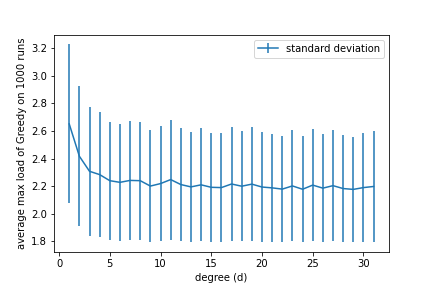
\includegraphics[scale=1.0]{Chapter4/Figs/Greedy_degree_analysis.png}
    \caption{Relating the degree of the graph to the performance of Greedy}
\end{figure}


We can see that indeed smaller degrees hurt Greedy, but after around $d=15$, the performance no longer improves. \NOTE{A}{Why does it perform worse on smaller degree graphs? Give some intuition. Also for why it plateaus. What effect might connectedness have on the performance? Does it matter e.g.\ for $d=2$ how many components the graph has? Future work...}



Even though Greedy is shown to be suboptimal in some cases, it is still by far the best strategy in the table (apart from DP), it proved to be an impossible challenge for RL to exploit the weaknesses of Greedy. In fact, for $n=m=32$, Deep Q-Learning is not even superior to the Random Strategy, which is equivalent to \OneChoice for any regular graph.\NOTE{D}{Why do you think this is the case? What could be going wrong here?}


\subsection{Deep Q-Learning analysis}

To better understand the difficulty in finding an optimal strategy, I extended the Cycle graph counterexample from Lemma \ref{lemma: greedy-suboptimal} to load vectors of the form $(0, a, 0, b)$, with the edge going between the $2$nd and $3$rd nodes. 


\begin{figure}[hbt!] \label{greedy-counterexample-analysed}
    \centering
    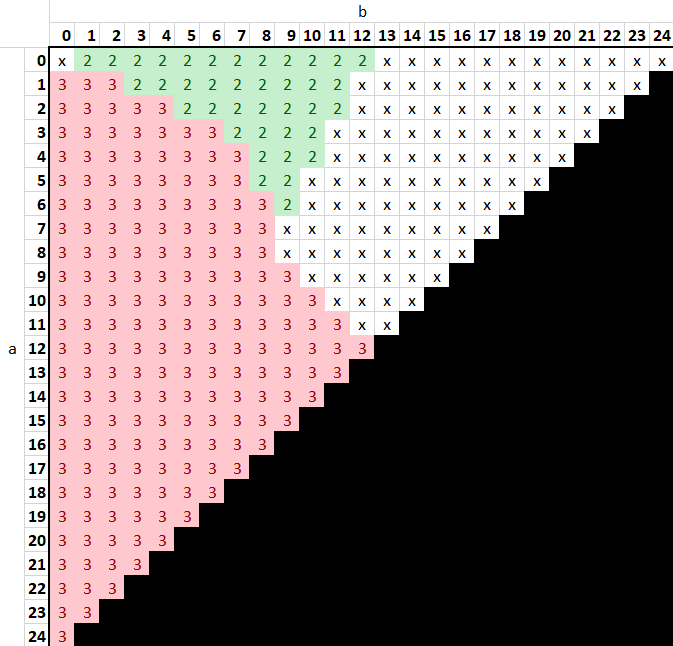
\includegraphics[scale=1.0]{Chapter4/Figs/0a0b_4_25_analysis.png}
    \caption{The optimal decisions for the Cycle graph with $n=4$, $m=25$, load vector $(0,a,0,b)$ and edge $2$-$3$. Green means choosing the $2$nd bin is better, red means choosing the $3$rd bin is better, and $x$ means they have the same expected score.}
\end{figure}


We can see in the figure\NOTE{D}{Which figure} that the green region contains the counterexamples to the Greedy strategy, but there is an even larger region where the greedy choice is correct, and characterising the shapes of the regions is difficult. By using a neighbourhood average based potential function for Deep Q-Learning, the agent is guided towards choosing $2$rd bin, and by using a graph-oblivious maximum load potential, the agent is guided towards choosing the $3$rd bin. Therefore, neither of the potential functions is perfect. For reference, here are the exact decisions made by the trained Deep Q-Learning strategy: \NOTE{A}{I am not sure if I should include it or not... It doesn't look very promising.}\NOTE{D}{Would it make sense to place thee figures side by side?}


\begin{figure}[hbt!] \label{greedy-counterexample-analysed-for-dqn}
    \centering
    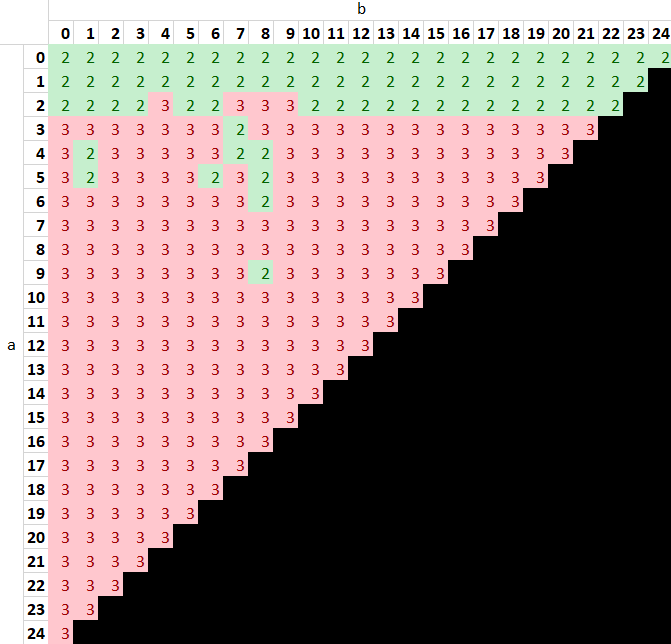
\includegraphics[scale=1.0]{Chapter4/Figs/0a0b_4_25_analysis_dqn.png}
    \caption{The decisions made by the Deep Q-Learning strategy for the Cycle graph with $n=4$, $m=25$, load vector $(0,a,0,b)$ and edge $2$-$3$. Green means choosing the $2$nd bin is better, red means choosing the $3$rd bin is better, and $x$ means they have the same expected score.}
\end{figure}
\NOTE{D}{Maybe the black color could be slightly lighter?}

We can see that the network couldn't learn the exact pattern, though there is some resemblance.


\subsubsection{Hyperparameter Analysis}

I present the hyperparameter importance analysis of $200$ runs for the Hypercube\NOTE{T}{very confusing? A hypercube with $4$ nodes is just a cycle, so it is better to only talk about cycles...} graph with $n=4$ and $m=25$, but the order is similar for other cases too.

\begin{figure}[hbt!] \label{graphical-two-choice-hyperparameter-importance}
    \centering
    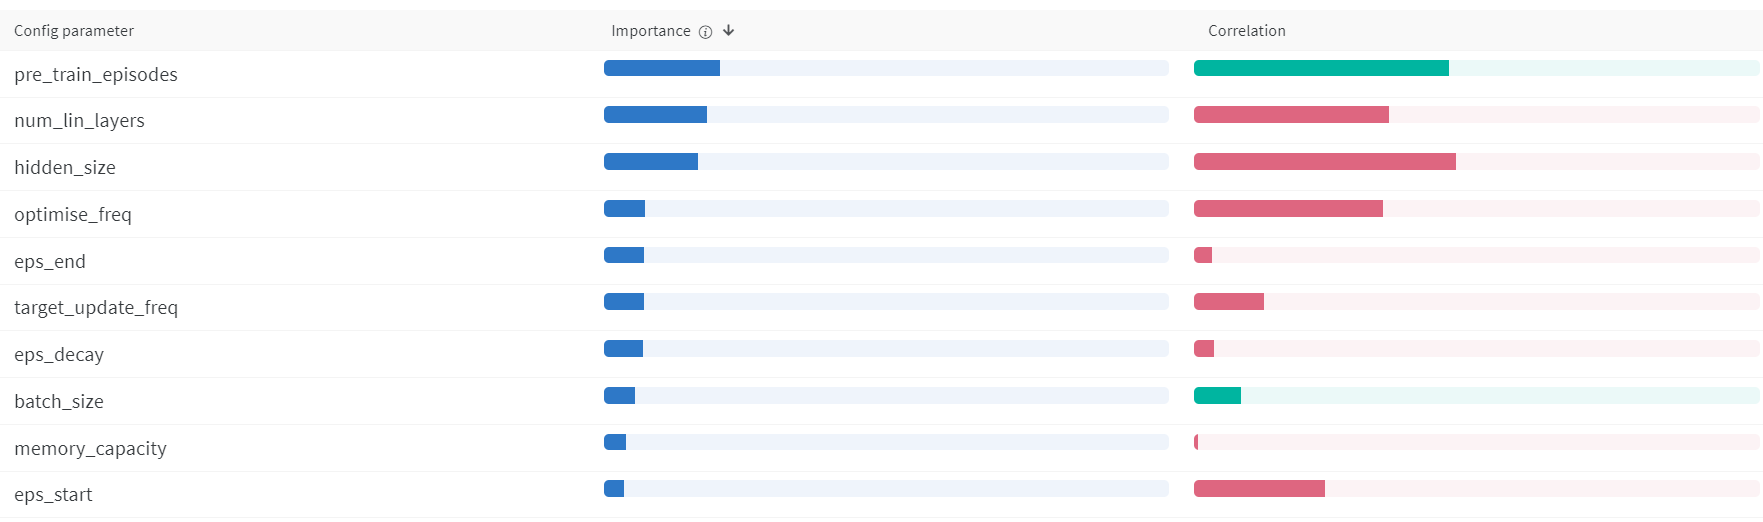
\includegraphics[scale=0.4]{Chapter4/Figs/graphical_two_choice_hypercube_4_25_importance.png}
    \caption{\GraphicalTwoChoice Hyperparameter Importance}
\end{figure}


Unlike the ``use\textunderscore threshold'' parameter for \TwoThinning, there is no very important hyperparameter (in fact, the trained scores are within a $0.4$ range for each analysed combination). The negative correlation of ``hidden\textunderscore size'' and ``num\textunderscore lin\textunderscore layers'' with the score shows that adding complexity to the neural network doesn't help.


\subsubsection{Training}

I present the training curve for the Hypercube graph with $n=4$ and $m=25$, but the pattern is similar for other cases too.


\begin{figure}[hbt!] \label{graphical-two-choice-hyperparameter-importance}
    \centering
    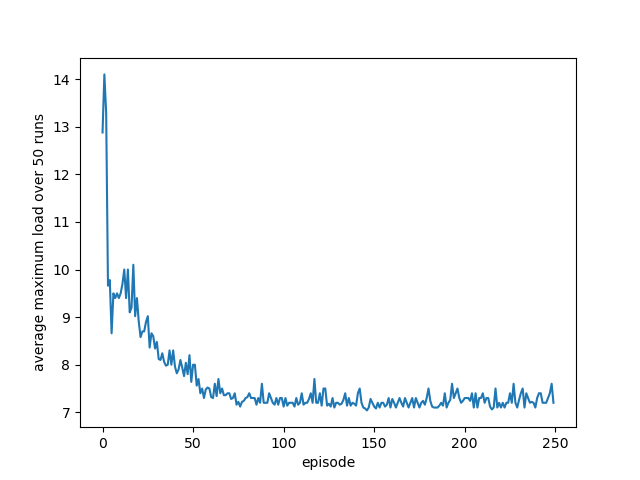
\includegraphics[scale=1.0]{Chapter4/Figs/training_progression_hypercube_4_25.png}
    \caption{\GraphicalTwoChoice Training Curve}
\end{figure}

We can see that unlike for \TwoThinning, the starting point is very poor, so that is a sharp increase initially. After $150$ episodes, the scores plateaus, even though the optimal expected maximum load is even lower.
